% =====================================================================
%  CAPÍTULO 6 — RESULTADOS E VALIDAÇÃO
% =====================================================================

\chapter{RESULTADOS E VALIDAÇÃO}
\label{cap:resultados}

Este capítulo apresenta os resultados do desenvolvimento do \argus{}, a
estratégia de validação adotada e as evidências de que o software atende aos
requisitos funcionais e não funcionais definidos.

\section{Estratégia de validação}
\label{sec:estrategia-validacao}

A validação do software foi conduzida em três frentes complementares:

\begin{itemize}
    \item \textbf{Validação funcional}: execução das funcionalidades do sistema
        em cenários reais de uso, verificando a conformidade com os requisitos
        funcionais (Tabela~\ref{tab:rf});
    \item \textbf{Validação experimental}: testes com equipamentos reais de
        ciclismo (rolos inteligentes e medidores de potência), aferindo
        estabilidade de conexão e latência de telemetria;
    \item \textbf{Validação de conformidade}: submissão dos arquivos
        \texttt{.fit} gerados a plataformas de análise (Strava e Intervals.icu)
        para comprovar a exatidão estrutural e estatística dos dados.
\end{itemize}

\section{Validação funcional}
\label{sec:validacao-funcional}

As funcionalidades implementadas foram exercitadas em ambiente real, cobrindo o
ciclo completo de treinamento: conexão com sensores, execução de sessões
livres e estruturadas, modos de evento e estúdio, gamificação, geração de
arquivos \texttt{.fit} e integrações com o Strava e o Intervals.icu. Os testes
foram conduzidos manualmente pelo autor ao longo do desenvolvimento, percorrendo
todas as funcionalidades descritas no Capítulo~\ref{cap:implementacao} sem
registro formal em planilha ou relatório de testes. A Figura~\ref{fig:screenshot-career}
ilustra o \textit{dashboard} de carreira com o gráfico PMC, e a
Figura~\ref{fig:screenshot-history} apresenta o histórico de atividades com as
métricas calculadas.

\begin{figure}[htbp]
    \centering
    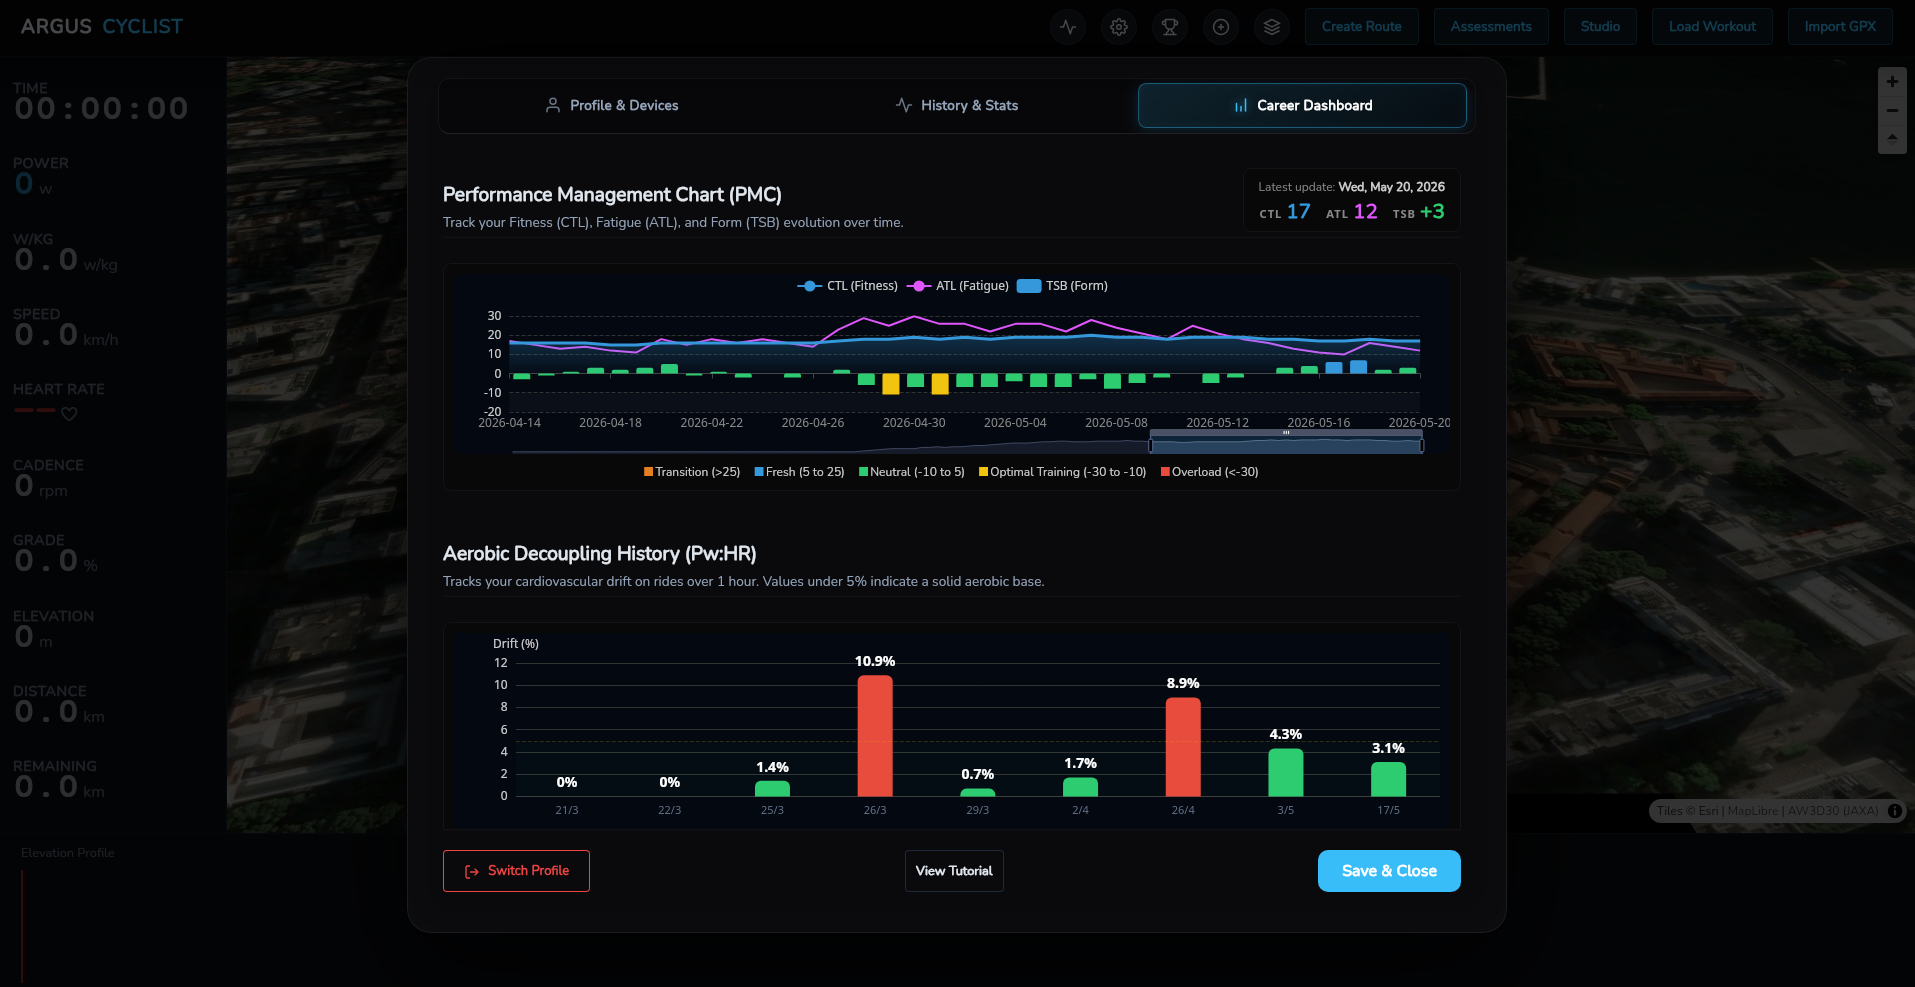
\includegraphics[width=0.85\textwidth]{figuras/screenshot-04-career}
    \caption{\textit{Dashboard} de carreira: PMC (CTL/ATL/TSB) e desvio cardiovascular}
    \label{fig:screenshot-career}
    \small Fonte: autoria própria.
\end{figure}

\begin{figure}[htbp]
    \centering
    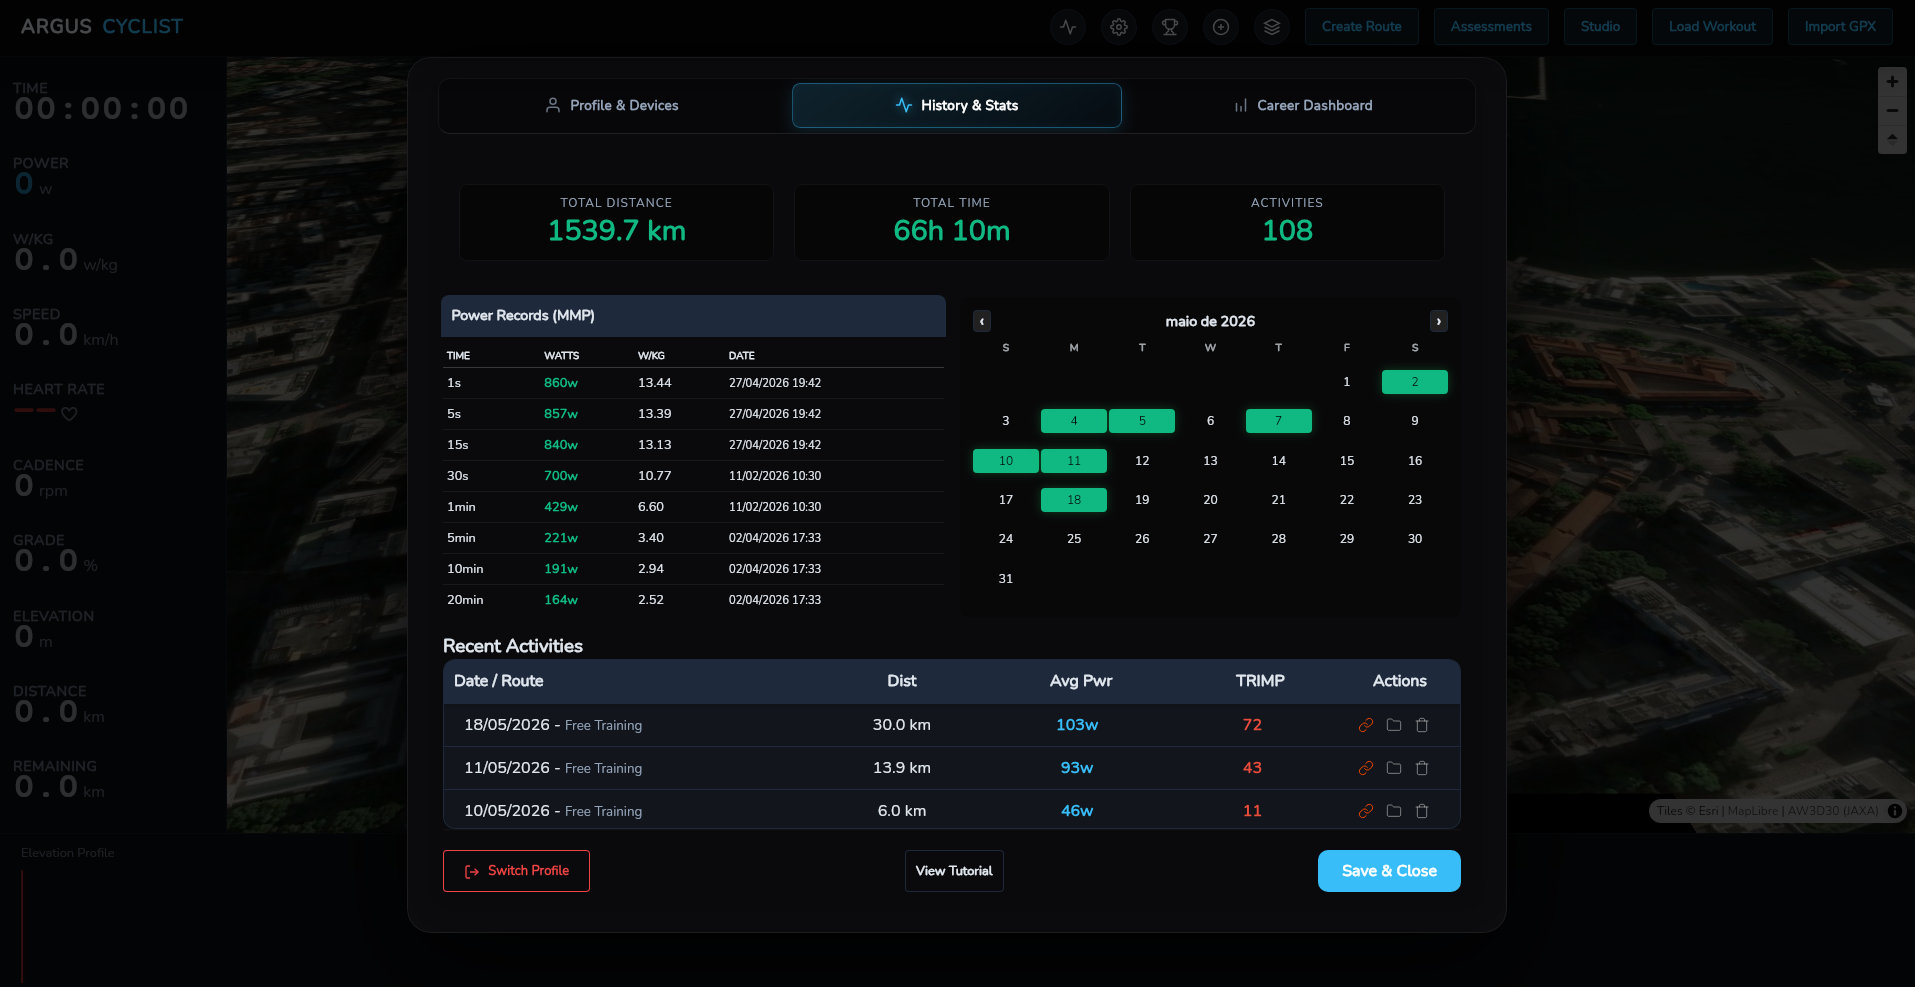
\includegraphics[width=0.85\textwidth]{figuras/screenshot-03-history}
    \caption{Histórico de atividades com métricas fisiológicas}
    \label{fig:screenshot-history}
    \small Fonte: autoria própria.
\end{figure}

\section{Validação experimental}
\label{sec:validacao-experimental}

A validação experimental foi realizada com equipamentos reais de ciclismo. O
\argus{} foi utilizado com o rolo inteligente (\textit{smart trainer}) ThinkRider
X2 MAX, a cinta de frequência cardíaca Cyplus H1 e um sensor de velocidade
(\textit{bike speed}). A comunicação também foi exercitada com a bicicleta
ergométrica Spinning SB 2000 Genis. Os testes foram conduzidos em três ambientes:
um notebook com Arch Linux, um PC com Windows 11 e um celular com Android. O
objetivo foi verificar a estabilidade das conexões BLE durante sessões contínuas
e a latência de telemetria entre a recepção do pacote e a atualização na
interface, comparando-a com o limite de \SI{150}{\milli\second} definido no
requisito RNF01.

\begin{table}[h]
    \centering
    \caption{Resultados da validação experimental}
    \label{tab:validacao}
    \small
    \begin{tabular}{
        >{\raggedright\arraybackslash}p{5.5cm}
        >{\centering\arraybackslash}p{2.6cm}
        >{\centering\arraybackslash}p{2.6cm}
        >{\centering\arraybackslash}p{3cm}
    }
        \toprule
        \textbf{Métrica} & \textbf{Alvo} & \textbf{Aferido} &
        \textbf{Conformidade} \\
        \midrule
        Latência de telemetria (sensor $\rightarrow$ tela) &
        $<$ \SI{150}{\milli\second} &
        $\sim$\SI{80}{\milli\second} &
        sim \\
        Estabilidade da conexão BLE (sessão contínua) &
        até 3~horas &
        3~horas sem desconexões &
        sim \\
        Consumo de memória do \textit{backend} (Go) &
        $<$ \SI{200}{\mega\byte} &
        $\sim$\SI{85}{\mega\byte} &
        sim \\
        \bottomrule
    \end{tabular}
\end{table}

A estabilidade da conexão BLE foi confirmada em sessões contínuas de até 3
horas de pedal, sem nenhuma desconexão do rolo inteligente ou da cinta de
frequência cardíaca. A latência de telemetria foi aferida em
$\sim$\SI{80}{\milli\second} (dentro do limite de \SI{150}{\milli\second}
definido no RNF01), e o consumo de memória do \textit{backend} foi de
$\sim$\SI{85}{\mega\byte} durante a simulação ativa (muito abaixo do limite
de \SI{200}{\mega\byte} do RNF04).

\section{Validação de conformidade dos dados (\texttt{.fit})}
\label{sec:validacao-conformidade}

Ao longo do desenvolvimento foram gerados mais de 200 arquivos \texttt{.fit}
no formato binário padrão Garmin/ANT+ \cite{garmin2024}. Todos foram exportados
para o Strava e o Intervals.icu (por meio da integração nativa de
\textit{upload}) e aceitos sem erros de importação, confirmando a
conformidade estrutural e estatística dos dados. Após a importação, as métricas
apresentadas por essas plataformas (distância, potência, elevação, frequência
cardíaca) conferiram com os valores registrados durante as sessões.

\section{Requisitos não funcionais}
\label{sec:rnf-atendidos}

A Tabela~\ref{tab:rnf} definiu os requisitos não funcionais do sistema. Todos
foram atendidos: a estabilidade de conexão (RNF03) foi confirmada em sessões
contínuas de até 3 horas sem desconexões; a portabilidade (RNF02) foi
exercitada com execução em Windows 11, Arch Linux e Android; a latência de
telemetria (RNF01) ficou em $\sim$\SI{80}{\milli\second}, inferior ao limite
de \SI{150}{\milli\second}; o consumo de memória (RNF04) foi de
$\sim$\SI{85}{\mega\byte}, abaixo do limite de \SI{200}{\mega\byte}; e o
processamento local e o licenciamento GPLv3 (RNF05 e RNF06) são garantidos
pela arquitetura e pela distribuição do código.

\section{Limitações e desafios}
\label{sec:limitacoes}

Durante o desenvolvimento, foram identificadas limitações e desafios que
orientam trabalhos futuros:

\begin{itemize}
    \item \textbf{Inferência da IA local}: a geração de planos de treino em
        dispositivos sem aceleração por GPU pode ser lenta, exigindo modelos
        quantizados e otimizações de \textit{prompt};
    \item \textbf{Validação com mais equipamentos}: a validação experimental
        concentrou-se em um conjunto específico de rolos e sensores, sendo
        desejável ampliar a cobertura de fabricantes e protocolos;
    \item \textbf{Disponibilidade de mapas offline}: a renderização do mapa 3D
        depende de \textit{tiles} obtidos da rede, havendo margem para caching
        local mais robusto em cenários totalmente \textit{offline};
    \item \textbf{Modo multiplayer}: o sistema é local e não contempla a
        interação social em tempo real entre atletas, uma funcionalidade
        central das plataformas comerciais.
\end{itemize}
